\section{Anhang}

\subsection{praktische Anwendungen der Redox Reaktionen}

\subsubsection{Inhalt} %maybe als Anhang?
\begin{itemize}
	\item galvanische Zellen
	\item  Batterien und Akkus
	\item  Brennstoffzellen
	\item  elektrolytische Verfahren
	

\end{itemize}

\subsection{Flüssigkristalle}

\subsubsection{Definition}
\begin{center}
	Aggregatszustand: flüssig und fest, flüsskristallin(trübe Farbe durch ZMK)
\end{center}
\begin{minipage}{0.48\linewidth}
	3 verschiedene flüssigkristalline Phasen:
	\begin{itemize}
  	  \item smektische Phase: \\
 	   	     kein Vorbeigleiten, Schichten
  	  \item nematische Phase: \\
  	  	     Vorbeigleiten möglich, ungeordnet
 	   \item cholesterische Phase: \\
	    	     Vorbeigleiten möglich, verdrehte Schichten
	\end{itemize}
	\hfill
\end{minipage}	
\begin{minipage}{0.48\linewidth}
	Eigenschaft für Phasen:
	\begin{itemize}
	    \item lange, stäbchenartige Moleküle (4x - 6x Molekülbreite)
	    \item starre Atomgruppen wie z.B. Benzol-Ringe, Doppel-, Dreifachbindungen
	    \item funktionelle Gruppe mit sehr starkem Dipolmoment (-CN-, -COOH)
	\end{itemize}
\end{minipage}




\subsubsection{TN-Zelle (Twisted Nematic)}
\begin{minipage}{0.48\linewidth}
	\begin{center}
		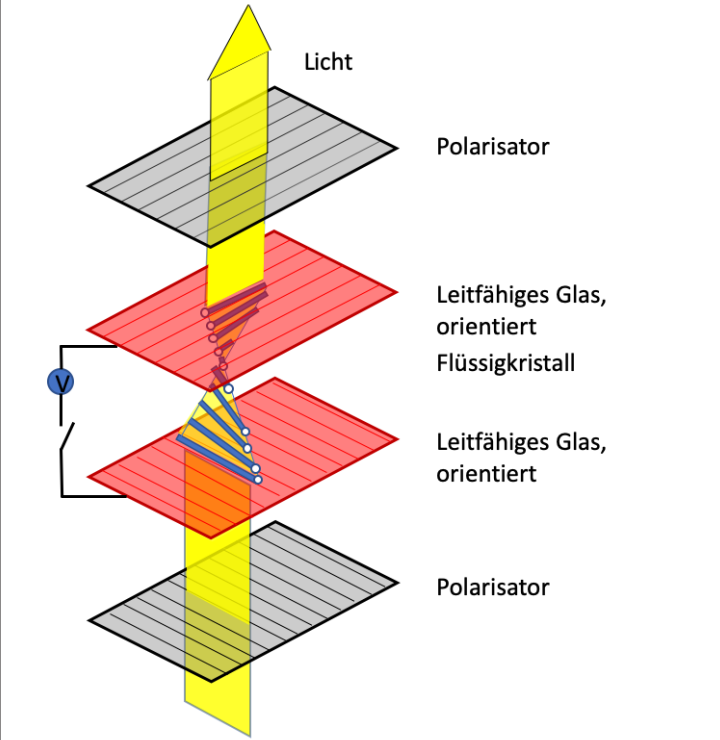
\includegraphics[width=0.8\linewidth]{images/TN-Zelle1.png}
		
		ohne angelegte Spannung   
	\end{center}
\end{minipage}
\hfill
\begin{minipage}{0.48\linewidth}
	\begin{center}
		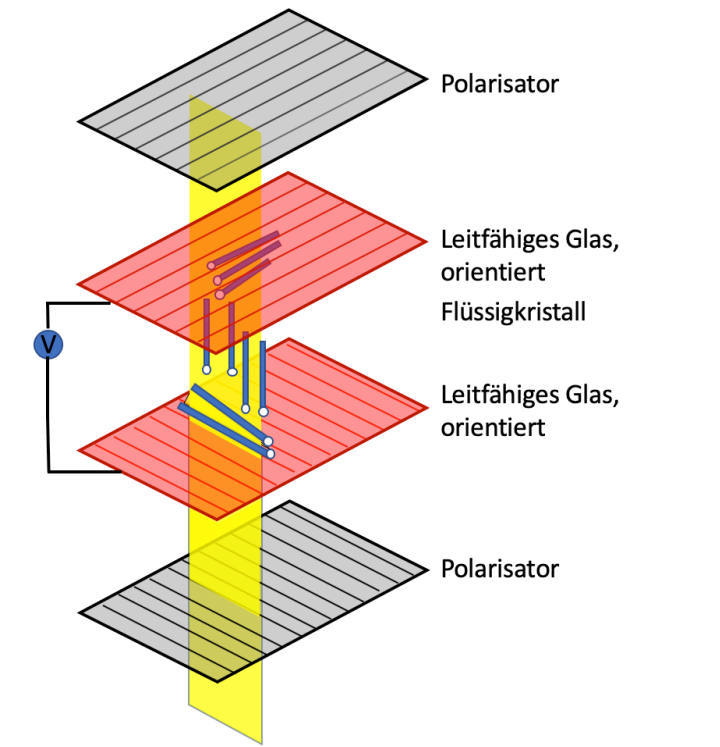
\includegraphics[width=0.8\linewidth]{images/TN-Zelle2.png} 
		
		mit angelegter Spannung 
	\end{center}
\end{minipage}



